\chapter{Gráficos do Experimento 1}

As Figuras \ref{fig:graphGC1-01}-\ref{fig:graphGC1-10} apresentam a evolução do VPL da melhor solução, da pior solução e a média da população das dez execuções do Algoritmo Genético Geracional Clássico durante o Experimento 1 duarnte a Etapa 1 ($AG^{CC-1}$).

\begin{figure}[H]
\centering
\includegraphics[scale=1]{apxA/aggc/1}
\caption{Primeira execução da versão clássica Algoritmo Genético Geracional com operadores de busca clássicos.}
\label{fig:graphGC1-01}
\end{figure}

\begin{figure}[H]
\centering
\includegraphics[scale=1]{apxA/aggc/2}
\caption{Segunda execução da versão clássica Algoritmo Genético Geracional com operadores de busca clássicos.}
\label{fig:graphGC1-03}
\end{figure}

\begin{figure}[H]
\centering
\includegraphics[scale=1]{apxA/aggc/3}
\caption{Terceira execução da versão clássica Algoritmo Genético Geracional com operadores de busca clássicos.}
\label{fig:graphGC1-03}
\end{figure}

\begin{figure}[H]
\centering
\includegraphics[scale=1]{apxA/aggc/4}
\caption{Quarta execução da versão clássica Algoritmo Genético Geracional com operadores de busca clássicos.}
\label{fig:graphGC1-04}
\end{figure}

\begin{figure}[htb]
\centering
\includegraphics[scale=1]{apxA/aggc/5}
\caption{Quinta execução da versão clássica Algoritmo Genético Geracional com operadores de busca clássicos.}
\label{fig:graphGC1-05}
\end{figure}


\begin{figure}[H]
\centering
\includegraphics[scale=1]{apxA/aggc/6}
\caption{Sexta execução da versão clássica Algoritmo Genético Geracional com operadores de busca clássicos.}
\label{fig:graphGC1-06}
\end{figure}

\begin{figure}[H]
\centering
\includegraphics[scale=1]{apxA/aggc/7}
\caption{Sétima execução da versão clássica Algoritmo Genético Geracional com operadores de busca clássicos.}
\label{fig:graphGC1-07}
\end{figure}

\begin{figure}[H]
\centering
\includegraphics[scale=1]{apxA/aggc/8}
\caption{Oitava execução da versão clássica Algoritmo Genético Geracional com operadores de busca clássicos.}
\label{fig:graphGC1-08}
\end{figure}

\begin{figure}[H]
\centering
\includegraphics[scale=1]{apxA/aggc/9}
\caption{Nona execução da versão clássica Algoritmo Genético Geracional com operadores de busca clássicos.}
\label{fig:graphGC1-09}
\end{figure}

\begin{figure}[H]
\centering
\includegraphics[scale=1]{apxA/aggc/10}
\caption{Décima execução da versão clássica Algoritmo Genético Geracional com operadores de busca clássicos.}
\label{fig:graphGC1-10}
\end{figure}

As Figuras \ref{fig:graphGRP1-01}-\ref{fig:graphGRP1-10} apresentam a evolução do VPL da melhor solução, da pior solução e a média da população das dez execuções do Algoritmo Genético de Regime Permanente Clássico durante o Experimento 1 da Etapa 1 ($AG^{RPC-1}$).

\begin{figure}[H]
\centering
\includegraphics[scale=1]{apxA/agrpc/1}
\caption{Primeira execução da versão clássica Algoritmo Genético de Regime Permanente com operadores de busca clássicos.}
\label{fig:graphGRP1-01}
\end{figure}

\begin{figure}[H]
\centering
\includegraphics[scale=1]{apxA/agrpc/2}
\caption{Segunda execução da versão clássica Algoritmo Genético de Regime Permanente com operadores de busca clássicos.}
\label{fig:graphGRP1-02}
\end{figure}

\begin{figure}[H]
\centering
\includegraphics[scale=1]{apxA/agrpc/3}
\caption{Terceira execução da versão clássica Algoritmo Genético de Regime Permanente com operadores de busca clássicos.}
\label{fig:graphGRP1-03}
\end{figure}

\begin{figure}[H]
\centering
\includegraphics[scale=1]{apxA/agrpc/4}
\caption{Quarta execução da versão clássica Algoritmo Genético de Regime Permanente com operadores de busca clássicos.}
\label{fig:graphGRP1-04}
\end{figure}

\begin{figure}[H]
\centering
\includegraphics[scale=1]{apxA/agrpc/5}
\caption{Quinta execução da versão clássica Algoritmo Genético de Regime Permanente com operadores de busca clássicos.}
\label{fig:graphGRP1-05}
\end{figure}

\begin{figure}[H]
\centering
\includegraphics[scale=1]{apxA/agrpc/6}
\caption{Sexta execução da versão clássica Algoritmo Genético de Regime Permanente com operadores de busca clássicos.}
\label{fig:graphGRP1-06}
\end{figure}

\begin{figure}[H]
\centering
\includegraphics[scale=1]{apxA/agrpc/7}
\caption{Sétima execução da versão clássica Algoritmo Genético de Regime Permanente com operadores de busca clássicos.}
\label{fig:graphGRP1-07}
\end{figure}

\begin{figure}[H]
\centering
\includegraphics[scale=1]{apxA/agrpc/8}
\caption{Oitava execução da versão clássica Algoritmo Genético de Regime Permanente com operadores de busca clássicos.}
\label{fig:graphGRP1-08}
\end{figure}

\begin{figure}[H]
\centering
\includegraphics[scale=1]{apxA/agrpc/9}
\caption{Nona execução da versão clássica Algoritmo Genético de Regime Permanente com operadores de busca clássicos.}
\label{fig:graphGRP1-09}
\end{figure}

\begin{figure}[H]
\centering
\includegraphics[scale=1]{apxA/agrpc/10}
\caption{Décima execução da versão clássica Algoritmo Genético de Regime Permanente com operadores de busca clássicos.}
\label{fig:graphGRP1-10}
\end{figure}